\documentclass{article}
\usepackage[T1]{fontenc}
\usepackage[utf8]{inputenc}
\usepackage[english]{babel}
\usepackage{tikz}
\usepackage{times}
\usetikzlibrary{calc,through,backgrounds,positioning,fit}
\usetikzlibrary{shapes,arrows,shadows,calendar}

\begin{document}
\begin{tikzpicture}[scale=1.6,inner sep=1cm]
\centering
\coordinate (A) at (0,0);
\coordinate (B) at (1.5,0.5);
\coordinate (C) at (1.5,-0.5);

\draw (A) node [above right] {$\varphi$};
\draw (A) node [below right] {$\varphi$};
\draw (1,0) node[right] {1};
\draw  (A) -- (B) -- (C)  --cycle;

\end{tikzpicture} \qquad \qquad \qquad
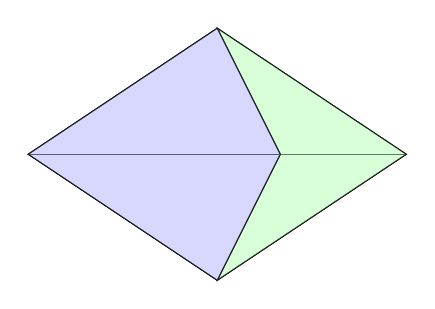
\begin{tikzpicture}[scale=1.6,inner sep=0.8cm]
\coordinate (A) at (0.5,0);
\coordinate (B) at (2,-1);
\coordinate (C) at (2,1);
\coordinate (D) at (3.5,0);
\coordinate (E) at (2.5,0);

\draw  (A) -- (B) -- (D) -- (C) --cycle;
\draw  (A) -- (D);
\draw  (B) -- (E) -- (C);

\filldraw [fill=green!30!white,opacity=0.5] (C) -- (D) -- (B) -- (E) -- cycle;
\filldraw [fill=blue!30!white,opacity=0.5] (C) -- (A) -- (B) -- (E) -- cycle;
\end{tikzpicture} \\\\
\input{zadanie_5.10_rys1.tex} \qquad \qquad \qquad
\input{zadanie_5.10_rys2.tex}  


\end{document}